\documentclass{sig-alternate}

\usepackage{listings}
\usepackage{algpseudocode}
\usepackage{algorithm}

% paper max 5 pages
% 1 page max appendix
% abstract max 250 words

\begin{document}

\title{Keywords Alternatives in lists of text}
\numberofauthors{2}
\author{
\alignauthor
Rik van Outersterp\\
       \affaddr{University of Twente}\\
       \affaddr{PO Box 217}\\
       \affaddr{Enschede, The Netherlands}\\
       \email{r.m.vanoutersterp@student.utwente.nl}
\alignauthor
Han van der Veen\\
        \affaddr{University of Twente}\\
       \affaddr{PO Box 217}\\
       \affaddr{Enschede, The Netherlands}\\
       \email{h.vanderveen-1@student.utwente.nl}
}
\date{27 January 2014}

\maketitle

\begin{abstract}
Using common text structure and Big Data, alternatives of subjects are extracted from many webpages. A common structure of lists in a text is used to determine these alternatives. These lists are combined into pairs and counted using MapReduce paradigm. The results are presented into a web application which can be searched on.
\end{abstract}

\category{H.3.3}{Information Storage and Retrieval}{Information Search and Retrieval}
\category{I.5.0}{Pattern Recognition}{General}

\keywords{Big Data, text analysis, text structure}

\section{Introduction}

\begin{quote}
``What if we can see immediately the alternatives for everything in the world?"
\end{quote}

Nowadays advertisers have a great influence on people. Using advertisements in media such as the Internet, television, and radio they try to convince people to buying certain products. However, advertisements can make the market seem smaller than it actually is. Not every company has the ability to advertise their product on the same scale as other companies.
That pushes people in certain directions, away from alternatives for which is advertised in a different way (e.g. another medium), in lesser extent, or not at all.

Our idea is that for every product in the world there is an alternative and that this alternative could be better than the original product. What we would like to do is to give people the option to find those alternatives and to compare them against each other and the original product. As advertisement is not always done for alternatives it can be difficult to find them. However, big data analysis can solve this problem.

In our research we choose to search only those alternatives in lists, because we think that will be sufficient to solve this problem. We use Big Data analysis on CommonCrawl data to retrieve alternatives for everything that is mentioned in the lists.

\subsection{Related work}
In a new moving science called Big Data, there are a lot of new techniques. Where Dean and Ghemawat~\cite{dean2008mapreduce} started with introducing MapReduce, new applications of MapReduce emerge. An overview of these techniques were given by Sakr et al.~\cite{sakr2013family}. In our paper we use techniques to extract the keywords which are related. Another method is to look for keywords in sentences. Zhu~\cite{Zhu2012} proposes a method for spotting keywords in large text, using a graph of the relations of words and the place of the words in the text to gather words into groups, and looking for keywords in those groups. This approach can also be applied when filtering the keywords. However, Big Data assumes that a lot of data will filter out the noise. 

Text structure is important in our approach. Delgado~\cite{delgado2002mining} uses structure of a text for extracting information of a text. For example, an episode is often mentioned with a format consisting the number of the season and the number of the episode (e.g. s03e12). Delgado does not use lists in texts, however he uses common structures in texts. 

In our approach we do not filter any of the results, but there may be a lot of the same which looks alike. We can filter them out by doing (as a post-filter) duplicate detection. Zhang~\cite{zhang2010efficient} uses partials of a sentence of duplicate detecting. Duplicate detection can also be used to clean the resultset.

\section{Method}
Our method is to analyse the common structure of lists in text assuming that they are relate to each other. The analysis of the alternatives is done through looking for lists that are mentioned in the pages itself. A list has a certain structure. It can be a sentence such as \emph{a, b or c} or \emph{x, y and z}. We use this common structure to find alternatives, since we assume that the listed elements are alternatives to each other.

We pack the crossproduct of the sentence \emph{x,y and z} into tuples. The tuples will be of the form \emph{(x,y), (y,z) and (z,x)}. Our mapper outputs the tuples with a concatenation of x and y. For example, \emph{x||y} is the emitted key with count 1. Algorithm~\ref{alg:mapper} is the mapper in pseudocode. We group on each pair. Our reducer does a sum on the occurences of the tuple. We assume that when a tuple has a high count, it is most likely to be related. 

\begin{algorithm}[t]
\caption{Mapper of Linker}
\label{alg:mapper}
\algrenewcommand\algorithmicfunction{\textbf{class}}
\algrenewcommand\algorithmicprocedure{\textbf{method}}
  \begin{algorithmic}[1]
    \Function{Mapper}{}
    \Procedure{Map}{$\textrm{docid }n, \textrm{doc }d$}
    \State $tuples \gets \textrm{pairs of }d$
    \ForAll{$\textrm{tuple }(a,b) \in tuples$}
	    \State $\textsc{Emit}(\textrm{string } \textrm{concat}(a,\textrm{||},b), \textrm{count }1 )$
    \EndFor
    \EndProcedure
    \EndFunction
  \end{algorithmic}
\end{algorithm}

\subsection{Text processing}
We extract our text with a simple regular expression, which can be found in the appendix~\ref{app:regex}. The list is splitted on \emph{comma}, \emph{and} or \emph{or}. Then the crossproduct of the pairs is emitted, taking in account that only one relation exists, such that \emph{(a,b)} is only emitted and not \emph{(b,a)}. This is achieved using a case-insensitive compare on a and b. Where a is lower than b, than a is before b and vise versa. These pairs are emitted into the MapReduce framework.

The MapReduce framework counts the results and the results are filtered with a small script to remove the results which have a count less than 25, which means that there the pair is reasonbly mentioned on the internet. These remaining results are loaded into a database through the parser. The database provides the basic interface for presenting the results.

\subsection{Expectations}
The expected result of the method is that on well known terms (e.g. Volkswagen) the results will be good. This is because that these terms are mentioned more often on the web. Furthermore, big terms are probably more related to other big terms. Also because these terms are mentioned more ofthen than other terms. The top results of each term will probably be related to other top results. 

\section{Results}
Our program has been tested on a sample of the dataset. The proposed test set for the Norvig Award  was not there anymore so we tested it on a subset of the CommonCrawl output (about 5GB of data)\footnote{with -maxfiles 50 switch}.

\subsection{Test set} 
We created 50 mappers and 1 reducer. The job was done in 31 minutes. Some of the jobs failed and that causes the long running time. If we use that for estimating what it takes using the full dataset, it takes about 100 days. However, on more data the cluster is faster, because every job can be runned directly after the other, so we think the job will be done in about 3 days. Our top results of our sample-subset is found in the appendix~\ref{app:testset}.

\begin{figure}[t]
	\label{img:screenSearch}
	\centering
	   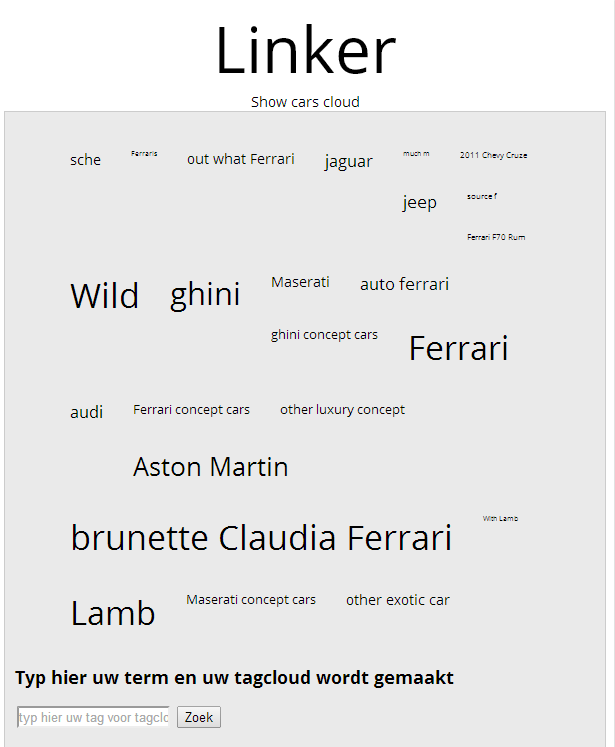
\includegraphics[width=0.5\textwidth]{screen_search_cloud.png}
	\caption{Search cloud for \emph{Ferrari}}
\end{figure}

\subsection{Full set} 
We had some errors with trying our solution on the fullset, but we did manage to run it on a set of 2,7TB of webdata. The full job took about 7 hours minutes and our result was about 97 million relational tuples\footnote{report of this job can be found on github}.

\subsection{Final results}
We created a tool for parsing the tuples and putting these in a database. The database can then be read through a simple web interface. In total almost 97 million combinations were found, which is equal to a database table of about 1.1 million rows. Note that we only have combinations with an amount of at least 25 times. The top three results in terms of combinations are: \emph{hit enter - search} and \emph{type - search}. All these combinations were found over 1.2 million times.

The alternatives are sometimes very good (i.e. the result is really an alternative for what we were searching for), but sometimes is really bad. The tool provides some basic relations, but not just alternatives like expected beforehand. For example, when searching on \emph{Ferrari} some other cars are mentioned, but also the phrase \emph{source f} which we could find no link with \emph{Ferrari} for.

\subsection{Killer result}
The tuples are all collected in a database and thanks to the MapReduce framework the tuples are already sorted alphabetically on the first word of the tuple (although with a SQL-query you can always sort the results in the way you prefer). The \emph{"killer result"} of our project is that of a simple webpage on which can be searched to find alternatives for the searched word. It should be clear that these alternatives are retrieved from the database.

The alternatives that are found for a search word are presented in a so called \emph{word cloud} (see Figure \ref{img:screenSearch}). Alternatives with a higher count (i.e. high amount of combinations of the searched word and the alternative) are displayed with a bigger font size and those with a lower count are displayed with a smaller font size.

Besides the search there is a special function available which only shows cars and their word clouds (see Figure \ref{img:screenCars}). This is done since the prototype of our system only consisted of cars and it gives a nice impression of what our system is capable of. Selecting a car results in a word cloud of the alternatives for that car, similar to the search function.

At the top of the webpage the top three tuples with the most references are listed, together with the total amount of references. These results are mentioned in details in the Results section.

\begin{figure}[t]
	\label{img:screenCars}
	\centering
		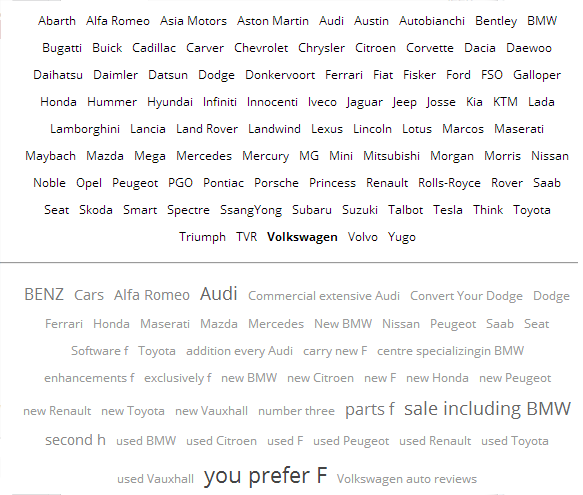
\includegraphics[width=0.5\textwidth]{screen_car_cloud.png}
		\caption{Word cloud for \emph{Volkswagen}}
\end{figure}

\section{Discussion}
The script have parsed many alternatives. The idea was to give an alternative for everything. We sort of did that, using the alternatives given in lists by users in html data. In our database we have pairs of relations. So, a relation with a high count is found many times in the html pages, thus likely to be related. 

There was a small bug that the matched sentence was splitted on \emph{or}, \emph{comma} or \emph{and}, thus the sentence \emph{parts for Audi} was splitted into \emph{parts f} and \emph{Audi}. Which is not correct. This was later fixed in the program. However, we did not manage to apply the fixed program on the full dataset, because we did not manage to run it again on the cluster. 

A shortcoming of our solution is that there are many duplicates. The duplicates generates a lot noise and needs to filtered out. With proper duplicate detection the dataset can be cleaned. Our solution is limited to short lists. An improvement could be to focus on the whole sentence. And apply the context of the sentence.

An improvement could be focusing on larger lists. With larger lists there is more information, thus more relations to be found. Extracting the essence of larger lists could result in better alternatives. 

\bibliographystyle{abbrv}
\bibliography{paper}

\balancecolumns
\appendix

\section{Sample Set Result}\label{app:testset}
First column is word a, second column is word b and after the semicolin is the occurence count of the tuple (a,b).
\begin{lstlisting}
broadcast||published;472
greeting cards||000 brochures;473
passw||Login with username;561
Bank Owned Homes||Columbus Ohio F;1630
Columbus Ohio F||eclosure;1630
eclosure||Columbus Ohio F;1630
\end{lstlisting}

\section{Regex}\label{app:regex}
\begin{lstlisting}
([a-z0-9\-\040]{3,25}[,])
([a-z0-9_\-\040]{3,25}[,]\s*){0,8}
([a-z0-9_\-\040]{3,25}(\s+(and|or)\s+)
[a-z0-9_\-\040]{3,25})
\end{lstlisting}

\section{Database structure}
\begin{lstlisting}
CREATE TABLE `dataset` (
  `a` varchar(255),
  `b` varchar(255),
  `c` int(11),
  INDEX(a), INDEX(b), INDEX(c)
) ENGINE=InnoDB DEFAULT;
\end{lstlisting}

\section{Files and data}\label{app:data}
Our project is public available on \emph{https://github.com/haneev/linker}. On github project page can be found how to install the application and how to use it. 

\balancecolumns

\end{document}
